\section*{Ejercicios}\label{ejercicios}
\addcontentsline{toc}{section}{Ejercicios}

\begin{ejercicio}
¿Qué mostrará en pantalla el siguiente programa
Python?

\begin{python}
def fred():
   print("Zap")

def jane():
   print("ABC")

jane()
fred()
jane()
\end{python}

a) Zap ABC jane fred jane\\
b) Zap ABC Zap\\
c) ABC Zap jane\\
d) ABC Zap ABC\\
e) Zap Zap Zap
\end{ejercicio}

\begin{ejercicio}Decid que es lo muestra por pantalla el siguiente programa:
\begin{python}
a = 4
def func (x):
    a=a+x
    return a

for cont in range(1,6):
    a=func(cont)
    print(a)
\end{python}

\end{ejercicio}

\begin{ejercicio}
Decid que es lo muestra por pantalla el siguiente programa:
\begin{python}
a = 0
b = 1

def func1 (a):
    b= func2(a+1)+1
	return b

def func2 (a):
	return (b+a)

for cont in range(1,6):
	b= b + func1 (a+1) + 1
    print(b)
\end{python}
\end{ejercicio}

\begin{ejercicio}\label{prod_sin_mult_funciones}
Recuerda el ejercicio \ref{prod_sin_mult}. Donde teniamos que 
implementar un programa que lea dos números enteros y diga si su producto es positivo, negativo, o cero \textbf{sin} llegar a realizar dicho producto. 

Los tests que teníamos que ejecutar ahí para probar que tu programa da las salidas esperadas eran: 
\begin{itemize}
\item primer numero es 0, 
\item segundo numero es 0, 
\item ambos números son 0, 
\item ambos números son positivos, 
\item ambos números son negativos, 
\item primer numero es negativo y segundo es positivo, 
\item primer numero es positivo y segundo es negativo.
\end{itemize}

Re-escribe tu solución para que tenga 2 funciones. Una función estéril \pythoninline{main()} que pide los datos al usuario y le comunica el resltado a traves de la consola. Una función productiva \pythoninline{prod_sin_mult} que implemente la funcionalidad deseada y devuelve el resultado.

Para testear tu solución llama a \pythoninline{main()} y ejecuta los mismos tests de antes en el ejercicio \ref{prod_sin_mult}:\\

\begin{Verbatim}[frame=single, label={\em ejemplos y posibles tests de ejecución}]
>>> main()
  Introduce el primer numero entero: 0
  Introduce el segundo numero entero: -1
  El producto es cero
>>> main() 
  Introduce el primer numero entero: 5
  Introduce el segundo numero entero: 0
  El producto es cero
>>> main() 
  Introduce el primer numero entero: 0
  Introduce el segundo numero entero: 0
  El producto es cero
>>> main() 
  Introduce el primer numero entero: 2
  Introduce el segundo numero entero: 7
  El producto es positivo
>>> main()  
  Introduce el primer numero entero: -4
  Introduce el segundo numero entero: -7
  El producto es positivo
>>> main()  
  Introduce el primer numero entero: -8
  Introduce el segundo numero entero: 3
  El producto es negativo
>>> main()  
  Introduce el primer numero entero: 10
  Introduce el segundo numero entero: -6
  El producto es negativo
\end{Verbatim}
\end{ejercicio}


\begin{ejercicio}\label{dados_rango_play_funciones}
Recuerda el ejercicio \ref{dados_rango_play}. Nos pide un programa para un simple juego de dos dados. El programa tenia que pedir al usuario los dos números de los dados d1 y d2 y decir si el jugador gana (7 o 11), pierde (2, 3 o 12) o si tiene otro chance (4, 5, 6, 8, 9 o 10).

Vamos a re-escribr tu solución para que tenga 3 funciones, una por cada una de las tareas del programa:

\begin{itemize}
    \item Una función estéril \pythoninline{main()} que se encarga de la interacción con el usuario.
    \item Una función productiva \pythoninline{dados_en_rango_correcto} que verifica que los dados están en el rango correcto
    \item Una función productiva \pythoninline{jugar} que solo llamamos cuando los dados están en el rango correcto y que aplica las reglas del juego
\end{itemize}

Para testear tu solución llama a \pythoninline{main()} y ejecuta los mismos tests de antes en el ejercicio \ref{dados_rango_play}:\\


\begin{Verbatim}[frame=single, label={\em example test execution of the program}]
>>> main()
  Valor del dado 1: 2
  Valor del dado 2: 4
  Tienes otra chance!
>>> main()
  Valor del dado 1: 1
  Valor del dado 2: 1
  Perdiste!
>>> main()
  Valor del dado 1: 6
  Valor del dado 2: 5
  Ganaste!
>>> main() 
  Valor del dado 1: 0
  Valor del dado 2: 3
  Error: dado 1 no tiene valor correcto
>>> main() 
  Valor del dado 1: 4
  Valor del dado 2: -8
  Error: dado 2 no tiene valor correcto
>>> main() 
  Valor del dado 1: 50
  Valor del dado 2: -4
  Error: dado 1 no tiene valor correcto
  Error: dado 2 no tiene valor correcto
\end{Verbatim}

\end{ejercicio}



\begin{ejercicio}
Vamos a automatizar la ejecución de los tests de Ejercicio \ref{prod_sin_mult_funciones}

\begin{python}
def prod_sin_mult(n1,n2):
    """
    Recibe dos números enteros y diga si su producto es positivo, negativo, o cero.
    SIN llegar a realizar dicho producto
    """
    #TU SOLUCION aqui

def test_prod_sin_mult():
    assert prod_sin_mult(0, -1) == "El producto es cero"
    assert prod_sin_mult(5, 0) == "El producto es cero"
    assert prod_sin_mult(0, 0) == "El producto es cero"
    assert prod_sin_mult(2, 7) == "El producto es positivo"
    assert prod_sin_mult(-4, -7) == "El producto es positivo"
    assert prod_sin_mult(-8, 3) == "El producto es negativo"
    assert prod_sin_mult(10, -6) == "El producto es negativo"
    
def main():
    n1 = int(input("Introduce primer numero: "))
    n2 = int(input("Introduce segundo numero: "))
    print(prod_sin_mult(n1,n2))
\end{python}
\end{ejercicio}


\begin{ejercicio}  
Vamos a automatizar la ejecución de los tests de Ejercicio \ref{dados_rango_play_funciones}

\begin{small}
\begin{python}
def dados_en_rango_correcto(d1, d2):
    """
    Verifica que dos dados estan dentro del rango correcto
    """
    #COMPLETAR
        
def jugar(d1,d2):
    """
    Aplica las reglas del juego, solo para dados en rango correcto
    """
    #COMPLETAR
  
def main():
    d1 = int(input("Valor del dado 1: "))
    d2 = int(input("Valor del dado 2: "))
    check_dados = dados_en_rango_correcto(d1, d2)
    if (dados_en_rango_correcto(d1, d2) == "Correcto"):
        print(jugar(d1,d2))
    else:
        print(check_dados)
  

def test_dados_en_rango_correcto():
    assert dados_en_rango_correcto(0, 3) == "Error: dado 1 no tiene valor correcto"
    assert dados_en_rango_correcto(5, -4) == "Error: dado 2 no tiene valor correcto"
    assert dados_en_rango_correcto(50, -4) == "Error: dados 1 y 2 no tienen valor correcto"
    assert dados_en_rango_correcto(2, 7) == "Error: dado 2 no tiene valor correcto"
    assert dados_en_rango_correcto(2, 6) == "Correcto"
    assert dados_en_rango_correcto(1, 1) == "Correcto"
    

def test_jugar():
    assert jugar(2, 4) == "Tienes otra chance!"
    assert jugar(1, 1) == "Perdiste!"
    assert jugar(6, 5) == "Ganaste!"    
\end{python}
\end{small}

\end{ejercicio}



\begin{ejercicio}
Escribir una función \pythoninline{my\_pow} que calcule $X^{n}$, tal que $X$ es un número real y $n$ un número entero positivo. Hay que escribir el programa \textit{sin} utilizar la función de librería pythoninline{Math.pow}. Esta función predefinida lo puedes usar en los pytests para chequear la salida de tu función, por ejemplo así:

\begin{small}
\begin{python}
import math
def test_my_pow():
    assert my_pow(2,0) == math.pow(2,0),   "caso Cardinalidad n = 0"
    assert my_pow(0,0) == math.pow(0,0),   "caso Dominio/Cardinalidad X=0 y n=0"
    assert my_pow(0,3) == math.pow(0,3),   "caso Dominio/Cardinalidad X=0, n>1"
    assert my_pow(5,10) == math.pow(5,10), "caso Dominio/Cardinalidad X>1, n>1"
    assert my_pow(-5,6) == math.pow(-5,6), "caso Dominio/Cardinalidad X<0, n>1"
\end{python}
\end{small}

Como vemos en el ejemplo, en Pytest es posible proporcionar un segundo parámetro opcional a la declaración assert. Este parámetro es una cadena de texto que se utiliza para proporcionar un mensaje personalizado en caso de que la afirmación falle.

El mensaje de error personalizado puede ayudar a identificar con mayor precisión la causa del fallo en la prueba. Puedes incluir información adicional relevante o describir la condición esperada que no se cumplió.
\end{ejercicio}



\begin{ejercicio}
Escribir una función (\pythoninline{change_string}) en python que dado un string \pythoninline{cad}, devuelve otro string en que la primera y el ultimo carácter de \pythoninline{cad} se han intercambiado.

También hay que incluir una funcion  pytest \pythoninline{test_change_string}, usando \pythoninline{assert} para probar tu función:

\begin{small}
\begin{python}
import pytest
def test_change_string1():
    assert change_string("") == ""              #Cardinalidad = 0
    assert change_string("z") == "z"            #Cardinalidad = 1
    assert change_string("tanja") == "aanjt"    #Cardinalidad > 1
    assert change_string("abbbba") == "abbbba"  #Orden
    assert change_string("12345") == "52341"    #Dominio
    assert change_string("!@ih&/") == "/@ih&!"  #Estructura
\end{python}
\end{small}

Si lo ejecutamos con pytest sale:

\begin{small}
\begin{python}
>>> %Run change_string.py
>>> !py.test change_string.py
============================= test session starts ==============================
platform darwin -- Python 3.7.9, pytest-6.1.2, py-1.9.0, pluggy-0.13.1
plugins: cov-4.0.0
collected 1 item

change_string.py .                                                       [100%]
============================== 1 passed in 0.01s ===============================
>>> 
\end{python}
\end{small}

Vemos que pytest considera \pythoninline{test_change_string1} con las 6 instruciones \pythoninline{assert} como 1 test. Lo podemos observar porque pone \pythoninline{collected 1 item} and 
\pythoninline{1 passed in 0.01s}.

Recuerda que la otra forma es usar \pythoninline{pytest.mark.parametrize}, lo explicamos otra vez abajo. OJO: si eso te parece todavía muy difícil o confusa, déjalo para más tarde.

\begin{small}
\begin{python}
import pytest
@pytest.mark.parametrize("testcase, entrada, salida_esperada",[
(1, "", ""),               #Cardinalidad = 0
(2, "z", "z"),             #Cardinalidad = 1
(3, "tanja", "aanjt"),     #Cardinalidad > 1
(4, "abbbba", "abbbba"),   #Orden
(4, "12345", "52341"),     #Dominio
(5, "!@ih&/", "/@ih&!")    #Estructura
])

def test_change_string2(testcase, entrada, salida_esperada):
    assert change_string(entrada) == salida_esperada, "caso {0}".format(testcase)
\end{python}
\end{small}


Si lo ejecutamos con pytest sale:

\begin{small}
\begin{python}
>>> %Run change_string.py
>>> !py.test change_string.py
============================= test session starts ==============================
platform darwin -- Python 3.7.9, pytest-6.1.2, py-1.9.0, pluggy-0.13.1
plugins: cov-4.0.0
collected 6 items

change_string.py ......                                                  [100%]

============================== 6 passed in 0.02s ===============================
>>> 
\end{python}
\end{small}

Vemos que pytest considera \pythoninline{test_change_string2} como 6 tests. Lo podemos observar porque pone \pythoninline{collected 6 items} and \pythoninline{6 passed in 0.02s}.

OJO: no olvida importar pytest así:
\pythoninline{import pytest}. Si no lo importas, el interpreter de Python no lo puede encontrar y te dirá: \texttt{NameError: name 'pytest' is not defined}.

\end{ejercicio}



\begin{ejercicio}
Escribir una función (\pythoninline{odd_values_string}) en python que dado un string $s$, devuelve otro string en que los caracteres en las posiciones con index impar se han eliminado. Tu función tiene que pasar tests los siguientes tests:


\begin{small}
\begin{python}
def test_odd_values_string():
    assert odd_values_string("") == ""
    assert odd_values_string("a") == "a"
    assert odd_values_string("aa") == "a"
    assert odd_values_string("abcd") == "ac"
    assert odd_values_string("abcde") == "ace"
    assert odd_values_string("12345") == "135"
    assert odd_values_string("&%$(agt.34") == "&$at3"
    assert odd_values_string("hola espacios  ") == "hl sais "
\end{python}
\end{small}   

Usando \pythoninline{pytest.mark.parametrize} quedaría así:

\begin{small}
\begin{python}
@pytest.mark.parametrize("testcase, entrada, salida_esperada",[
(1, "", ""),                       #Cardinalidad = 0
(2, "a", "a"),                     #Cardinalidad = 1 (0 letras en posición impar)
(3, "aa", "a"),                    #Cardinalidad = 2 (1 letra en posición impar)
(4, "abcd", "ac"),                 #Cardinalidad 2 posiciones impar, 5 letras
(5, "abcde", "ace"),               #Cardinalidad 2 posiciones impar, 5 letras
(6, "12345", "135"),               #Dominio, string con digitos
(7, "&%$(agt.34", "&$at3"),        #Estructura, string con signos
(8, "hola espacios  ", "hl sais ") #Estructura, string con espacios
])

def test_odd_values_string(testcase, entrada, salida_esperada):
    assert odd_values_string(entrada) == salida_esperada,\
           "caso {0}".format(testcase)
\end{python}
\end{small}

\end{ejercicio}

\begin{ejercicio}
Escribir una función \pythoninline{mi_raiz} que calcule la raíz cuadrada de un número $n$, aplicando el método babilónico. Este método consiste en el cálculo de la sucesión $S$:
\begin{center}
$S = \lbrace s_{i} \rbrace ^{\infty}_{i=0}= s_{0} , s_{1} , s_{2} , \dots , s_{\infty}$ donde $: s_{0} = 2 $    y   $ s_{i+1} = \frac {s_{i} + n/s_{i}}{2}$
\end{center}
Cada uno de los términos $s_{i}$ de la serie es una aproximación a $\sqrt{n}$. Evidentemente, el último de los términos calculados será la mejor aproximación. Se calculará un nuevo término $s_{i+1}$ siempre y cuando se cumpla $|s_{i-1} - s_{i} | > 10^{-8}$ .


Puedes usar \pythoninline{math.sqrt} como resultado esperado en tus casos de test. Sin embargo, hay que tener en cuenta que comparar flotantes para la igualdad es un poco complicado debido a problemas de redondeo y precisión.
Podemos comparar que la diferencia entre lo que sale de nuestra función y el \pythoninline{math.sqrt} es menor a por ejemplo $10^{-2}$

\begin{small}
\begin{python}
def test_mi_raiz():
    assert abs(mi_raiz(2) - math.sqrt(2)) < 10**-2, "caso n=2"
    assert abs(mi_raiz(4) - math.sqrt(4)) < 10**-2, "caso n=4"
    assert abs(mi_raiz(7) - math.sqrt(7)) < 10**-2, "caso n=7"
    assert abs(mi_raiz(25) - math.sqrt(25)) < 10**-2, "caso n=25"
    assert abs(mi_raiz(200) - math.sqrt(200)) < 10**-2, "caso n=200"
    assert abs(mi_raiz(1234) - math.sqrt(1234)) < 10**-2, "caso n=1234"
\end{python}
\end{small}
\end{ejercicio}



\begin{ejercicio}
Escribir una función \pythoninline{my\_coseno} que dado un valor real $x > 0$, calcule el coseno de $x$ mediante la siguiente serie:
$$cos(x)=\sum_{i=0}^{\infty}(-1)^{i}\frac{x^{2i}}{(2i)!}= 1 - \frac{x^{2}}{2!} + \frac{x^{4}}{4!} - \dots$$
Se deben calcular términos de la serie mientras el valor absoluto de cada término sea superior a $10^{-7}$.

OJO: Si queremos calcular el coseno de 45 grados usando nuestra función \pythoninline{my\_coseno}, primero tenemos que convertir 45 grados en radianes. Afortunadamente, el módulo matemático de Python tiene una función llamada \pythoninline{math.radians()} que realiza la conversión de ángulos antes.

Aquí puedes usar \pythoninline{math.cos} como resultado esperado en tus casos de test. De nuevo hay que tener en cuenta que comparar flotantes para la igualdad es complicado debido a problemas de redondeo y precisión.
\end{ejercicio}

\begin{ejercicio}
Escribir una función que dado un valor real $x > 0$, calcule el arco-tangente de $x$ mediante la siguiente serie:
$$arctan(x) = \sum_{n=0}^{\infty}(-1)^{i}\frac{x^{2n+1}}{2n+1}= x - \frac{1}{3}x^{3}+\frac{1}{5}x^{5}-\frac{1}{7}x^{7}+\dots$$
Se deben calcular términos de la serie mientras el valor absoluto de cada término sea mayor que $10^{-7}$.

Recuerda usar \pythoninline{math.radians()}. Puedes usar \pythoninline{math.atan} como resultado esperado en tus casos de pytest.
\end{ejercicio}



\begin{ejercicio}
\index{objeto!de función}
\index{función!objeto de}

Un objeto de función es un valor que puedes asignar a una variable o
pasarlo como argumento.  Por ejemplo, \verb"hacer_2veces" es una función
que toma un objeto de función como argumento y lo llama dos veces:

\begin{python}
def hacer_2veces(f):
    f()
    f()
\end{python}

Aquí hay un ejemplo que utiliza \pythoninline{hacer_2veces} para llamar a una función
con nombre \pythoninline{imprimir_spam} dos veces.

\begin{python}
def imprimir_spam():
    print('spam')

hacer_2veces(imprimir_spam)
\end{python}

\begin{enumerate}

\item Escribe este ejemplo en un script y pruébalo.

\item Modifica \pythoninline{hacer_2veces} para que tome dos argumentos, un
objeto de función y un valor, y llame a la función dos veces,
pasando al valor como argumento.

\item Recuerda y copia la definición de
\pythoninline{muestra_dos_veces}, presentada previamente en este tema, a tu script.

\begin{python}[frame=single]
def muestra_dos_veces(bruce):
    print(bruce)
    print(bruce)
\end{python}


\item Usa la versión modificada de \pythoninline{hacer_2veces} para llamar a
\pythoninline{muestra_dos_veces} dos veces, pasando a \pythoninline{'spam'} como argumento.

\item Define una nueva función llamada
\pythoninline{hacer_4veces} que tome un objeto de función y un valor
y llame a la función cuatro veces, pasando al valor
como argumento.  Debería haber solo
dos sentencias en el cuerpo de esta función, no cuatro.

\end{enumerate}

%Solution: \url{http://thinkpython2.com/code/do_four.py}.

\end{ejercicio}

\begin{ejercicio}
\label{anagram}
\index{anagrama}
%
Dos palabras son anagramas si puedes reordenar las letras de una
para escribir la otra.  Escribe una función llamada \pythoninline{es_anagrama}
que tome dos cadenas y devuelva \pythoninline{True} si son anagramas.

En la pagina \url{https://www.ejemplos.co/50-ejemplos-de-anagramas/} puedes encontrar ejemplos de anagramas para escribir tus pytests.


\end{ejercicio}

\begin{ejercicio}
Escribir una función  que, dado un número entero $n$ mayor que cero,
devuelve una lista de los múltiplos de 3 que hay entre 3 y $n$. Escribe otra función que, dado un número entero $n$ mayor que cero, devuelve una lista de los divisores de $n$. Prueba tus funciones con pytest, por ejemplo:

\begin{python}
@pytest.mark.parametrize('testcase, entrada, salida_esperada',[
    (1, 10, [3, 6, 9]),
    (2, 0, []),
    (3, 1, []),
    (4, -5, []),
    (5, 12, [3, 6, 9, 12]),
    (6, 3, [3])
    ])
def test_multiplos_de_3(testcase, entrada, salida_esperada):
    assert multiplos_de_3(entrada)==salida_esperada, 'caso {0}'.format(testcase)

@pytest.mark.parametrize('testcase, entrada, salida_esperada',[
    (1, 10, [1, 2, 5, 10]),
    (2, 18, [1, 2, 3, 6, 9, 18]),
    (3, 1, [1]),
    (4, -5, []),
    (5, 12, [1, 2, 3, 4, 6, 12]),
    (6, 0, [])
    ])
def test_divisores_de(testcase, entrada, salida_esperada):
    assert divisores_de(entrada)==salida_esperada, 'caso {0}'.format(testcase)
\end{python}

Ahora, usa estas funciones para escribir un programa \pythoninline{main} que pide un numero mayor que cero al usuario a través del teclado que devuelve el siguiente:\\

\begin{Verbatim}[frame=single]
>>> %Run 
  Teclea un numero entero mayo a cero: 1
  No hay multiplos de 3
>>> %Run 
  Teclea un numero entero mayo a cero: 2
  No hay multiplos de 3
>>> %Run 
  Teclea un numero entero mayo a cero: 3
  multiplo = 3 divisores del 3 = [1, 3]
>>> %Run 
  Teclea un numero entero mayo a cero: 13
  multiplo = 3 divisores del 3 = [1, 3]
  multiplo = 6 divisores del 6 = [1, 2, 3, 6]
  multiplo = 9 divisores del 9 = [1, 3, 9]
  multiplo = 12 divisores del 12 = [1, 2, 3, 4, 6, 12]
>>> 
\end{Verbatim}


\end{ejercicio}

\begin{ejercicio}
Escribir una función (\pythoninline{letraDNI}) que, dado un número de DNI, devuelva la letra que le corresponde.
%
El algoritmo para calcular la letra de control de un DNI es el siguiente:
\begin{itemize}
\item Calcula el resto de dividir el n\'umero por 23
\item Se obtiene la letra, utilizando el resto como
índice de la siguiente tabla:\\
\end{itemize}

  \begin{tabular}{|c|c|c|c|c|c|c|c|c|c|c|c|c|}
    \hline
    RESTO & 0 & 1 & 2 & 3 & 4 & 5 & 6 & 7 & 8 & 9 & 10 & 11  \\ \hline
    LETRA & T & R & W & A & G & M & Y & F & P & D & X & B  \\ \hline
  \end{tabular}
  
  \begin{tabular}{|c|c|c|c|c|c|c|c|c|c|c|c|}
    \hline
    RESTO & 12 & 13 & 14 & 15 & 16 & 17 & 18 & 19 & 20 & 21 & 22 \\ \hline
    LETRA & N & J & Z & S & Q & V & H & L & C & K & E  \\ \hline
  \end{tabular}\\

Completa la siguiente tabla con la cantidad de filas que ves necesario para diseñar tu conjunto de tests y ejecuta los tests automáticos con pytest.\\

\begin{tabular}{|l|l|l|}
\hline
caso de test número & entrada & salida esperada   \\ \hline\hline
1 & \verb@                      @ & \verb@                       @\\
2 & & \\
3 & & \\
4 & & \\
5 & & \\
6 & & \\
\hline
\end{tabular}


\end{ejercicio}

\begin{ejercicio}
Diseña una función que dado una cadena de texto, devuelve la cantidad de números que aparecen en la cadena. Nota: Con número no queremos decir dígito, sino número propiamente dicho, es decir, secuencia de dígitos. La cadena `un 1, un 201 y 2 unos', por ejemplo, tiene 3 números: el 1, el 201 y el 2.\\

\begin{Verbatim}[frame=single, label={\em ejemplo de ejecuciones}]
>>> nums_en_string("un 1, un 201 y 2 unos")
  3
>>> nums_en_string("sin numeros")
  0
>>> nums_en_string("2345543")
  1
\end{Verbatim}

Escribe pytests para probar tu función de forma automatizado.

\end{ejercicio}

\begin{ejercicio}

Implementa un modulo con un \pythoninline{main} que lea de teclado una cadena que representa un número binario. Si algún carácter de la cadena es distinto de 0 o 1, el programa advertirá al usuario de que la cadena introducida no representa un número binario y pedirá de nuevo la lectura de la cadena. Finalmente, el \pythoninline{main} mostrará el valor entero decimal del número binario introducido.

En el \pythoninline{main} tienes que usar 2 funciones que tienes que definir y testear con pytest en tu modulo:

\begin{itemize}
\item \pythoninline{check_si_es_binario} que dado una cadena de texto devuelve \pythoninline{True} si la cadena esta compuesto por solo 0 y 1, y si no devuelve \pythoninline{False}
\item \pythoninline{convertir} para convertir una cadena en formato binario (i.e. solo 0 y 1) a formato decimal.
\end{itemize}

¿Qué casos de test ejecutarías para probar bien tu main?
¿Y para las 2 funciones? Implementa los tests con pytest.


\end{ejercicio}

\begin{ejercicio}
Implementar una función \pythoninline{fib(n)}
que devuelve una lista con los primeros \pythoninline{n} números de 
Fibonacci. Si \pythoninline{n==0}, la función tiene que devolver la lista 
\pythoninline{[1]}, si \pythoninline{n==1}, la función tiene que devolver la lista\pythoninline{[1,1]}. Cuando \pythoninline{n<1}, entonces hay que empezar con la lista \pythoninline{[1,1]} y añadir el siguiente numero Fibonacci sumando los números anteriores en la lista.

Por ejemplo tecleando:\\

\begin{Verbatim}[frame=single]
>>> print(fib(0))
  [1]
>>> print(fib(1))
  [1, 1]
>>> print(fib(2))
  [1, 1, 2]
>>> print(fib(12))
  [1, 1, 2, 3, 5, 8, 13, 21, 34, 55, 89, 144, 233]
\end{Verbatim}

¡No olvida tus pytests para automatizar los tests!

\end{ejercicio}

\begin{ejercicio}
Escribir una función Python \pythoninline{borrar_negativos} que recibe como argumento una lista y devuelve la misma lista pero sin los elementos negativos.\\

\begin{Verbatim}[frame=single]
>>> borrar_negativos([0,-1,-11,2,33,-100,5])
  [2, 33, 5]
>>> borrar_negativos([-1,-11,-3])
  []
>>> borrar_negativos([4,68,111])
  [4, 68, 111]
\end{Verbatim}

Ejecuta más tests automáticos con pytest. No olvides un tests para la lista vacía y la lista con 1 elemento.

\end{ejercicio}

\begin{ejercicio}
Escribe una función (\pythoninline{posMax}) que dada una lista no vacía devuelva la posición donde se encuentra su valor máximo.
Después, completa la tabla de abajo con la cantidad de filas que ves necesario para diseñar tu conjunto de tests y ejecuta los tests automáticos con pytest. Esta vez no hace falta testear la lista vacía, porque el enunciado dice claramente que tu función solo tiene que funcionar para una lista no vacía.\\

\begin{tabular}{|l|l|l|}
\hline
caso de test número & entrada & salida esperada   \\ \hline\hline
1 & \verb@                      @ & \verb@                       @\\
2 & & \\
3 & & \\
.... & & \\
\hline
\end{tabular}


\end{ejercicio}

\begin{ejercicio}
Escribir una función que dada una lista de palabras y una palabra devuelva el número de veces que aparece dicha palabra en la lista. Después, completa la tabla con la cantidad de filas que ves necesario para diseñar tu conjunto de tests y ejecuta los tests automáticos con pytest.\\

\begin{tabular}{|l|l|l|}
\hline
caso de test número & entrada & salida esperada   \\ \hline\hline
1 & \verb@                      @ & \verb@                       @\\
2 & & \\
3 & & \\
.... & & \\
\hline
\end{tabular}

\end{ejercicio}

\begin{ejercicio}
Diseña una función (\pythoninline{miSplit}) que obtiene una cadena y devuelve una lista con todas sus palabras en minúsculas. La lista devuelta no debe contener palabras repetidas. 
No puedes usar el \pythoninline{split} predefinido de Python.
Por ejemplo, ante la cadena:\\

\begin{Verbatim}[frame=single]
>>> miSplit('Una frase formada con palabras. Otra frase con otras palabras.')
  ['una', 'frase', 'formada', 'con', 'palabras', 'otra', 'otras']
>>> miSplit('Hi! Helloooo HI')
  ['hi', 'helloooo']
\end{Verbatim}

Para diseñar tu conjunto de tests que tienes que ejecutar de forma automáticos con pytest piensa en casos:

\begin{itemize}[nosep]
    \item que la cadena es vacía
    \item que la cadena tiene signos de puntuación, como  \verb|,;.:-¿?+*()!¡|
    \item que la cadena termine con un punto
    \item que la cadena no termine con un punto
    \item que la cadena tiene números
    \item que la cadena tiene palabras repetidos, pero unos tiene mayúsculas y otras no (por ejemplo: \pythoninline{'HOla hola hoLa'}
    \item que la cadena tiene más de 1 espacio entre palabras
    \item etc.
\end{itemize}


\end{ejercicio}

\begin{ejercicio}
Escribir una función que dada una lista de números devuelva otra lista sin los números impares. 
Después, completa la tabla con la cantidad de filas que ves necesario para diseñar tu conjunto de tests y ejecuta los tests automáticos con pytest.\\

\begin{tabular}{|l|l|l|}
\hline
caso de test número & entrada & salida esperada   \\ \hline\hline
1 & \verb@                      @ & \verb@                       @\\
2 & & \\
3 & & \\
.... & & \\
\hline
\end{tabular}

\end{ejercicio}

\begin{ejercicio}
Escribir una función que dada una lista de números devuelva otra lista sin elementos repetidos. Después, completa la tabla con la cantidad de filas que ves necesario para diseñar tu conjunto de tests y ejecuta los tests automáticos con pytest.\\

\begin{tabular}{|l|l|l|}
\hline
caso de test número & entrada & salida esperada   \\ \hline\hline
1 & \verb@                      @ & \verb@                       @\\
2 & & \\
3 & & \\
.... & & \\
\hline
\end{tabular}


\end{ejercicio}

\begin{ejercicio}
Escribir un modulo con tres funciones y sus pytest sobre matrices: \pythoninline{sum\_of\_diagonal}, \pythoninline{create\_matriz} y \pythoninline{multiplicar}.

1) La primera función es (\pythoninline{sum\_of\_diagonal}) que dado una matriz $m$ de integers calcula la suma de los integers que están en el diagonal. Tu función tiene que comprobar que la matriz es cuadrada y efectivamente tiene un diagonal para sumar. Por ejemplo:

$
{\texttt{tt sum\_of\_diagonal}}(
\begin{bmatrix}
    1 & 2 & 3 & 4 \\
    2 & 4 & 6 & 1 \\
    0 & 5 & 8 & 2 \\
    2 & 9 & 6 & 3 \\
\end{bmatrix})
 = 16
$, $\;\;$
$
{\texttt{sum\_of\_diagonal}}(
\begin{bmatrix}
    1 & 5   \\
    3 & 4  \\
\end{bmatrix})
 = 5
$

Tu función tiene que pasar los siguientes tests:

\begin{small}
\begin{python}
@pytest.mark.parametrize("testcase, input, output",[
(1, [[1,2,3],[4,5,6],[7,8,9]], 15),
(2, [[1,0,1],[1,1,0],[1,1,1]], 3),
(3, [[2,0],[0,2]], 4),
(4, [[2,0],[0,2,3]], "matriz no es cuadrada"),
(5, [], 0)]

def test_sum_of_diagonal(testcase, input, output):
    assert sum_of_diagonal(input) == output,\
           "caso {0}".format(testcase)
\end{python}
\end{small}

2) Después, escribimos una función (\pythoninline{create\_matriz}) que dado dos números $n$ y $m$ devuelve una lista que representa una matriz con $n$ filas y $m$ columnas con todos el valor 0.

$
{\texttt{create\_matrix}}(3,4) = 
\begin{bmatrix}
    0 & 0 & 0 & 0 \\
    0 & 0 & 0 & 0 \\
    0 & 0 & 0 & 0 \\
\end{bmatrix})
$

Diseñar un conjunto de casos de test y automatizarlos con el pytest.

3) La tercera función es para (\pythoninline{multiplicar}), dado dos matrices $m_1$ y $m_2$ devuelve $m_1 \times m_2$. Recuerda\footnote{\url{https://es.wikipedia.org/wiki/Multiplicación_de_matrices}}
que solo podemos multiplicar 2 matrices si el número de columnas de la matriz $m_1$ es igual al número de filas de la matriz $m_2$.\\

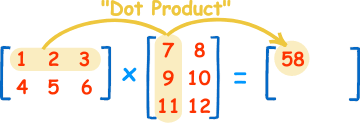
\includegraphics[width=0.5\textwidth]{book/Spanish/05_Funciones/images/mult-matrix.png}

Tu función tiene que pasar los siguientes tests:

\begin{small}
\begin{python}
@pytest.mark.parametrize("testcase, input1, input2, output",[
(1, [[12,7,3], 
     [4, 5,6], 
     [7, 8,9]],
    [[5,8,1,2],
     [6,7,3,0],
     [4,5,9,1]],
    [[114, 160,  60, 27], 
     [ 74,  97,  73, 14], 
     [119, 157, 112, 23]]
),
(2, [[12,7,3, 0], 
     [ 4,5,6,12], 
     [ 6,7,8, 9]
    ],
    [[8,5,8,1,2],
     [6,9,7,3,0],
     [4,5,9,1,0],
     [4,5,9,1,0]
    ],
    [[150, 138, 172, 36, 24], 
     [134, 155, 229, 37, 8], 
     [158, 178, 250, 44, 12]
    ]
),
(3, [], [], []
),
(4,[[]],[[]], "no se pueden multiplicar"
),
(5, [[]],[[[]]], "no se pueden multiplicar"
),
(6, [[[]]],[[]], [[]]
)
])

def test_multiplicar(testcase, input1, input2, output):
    assert multiplicar(input1, input2) == output, 
           "caso {0}".format(testcase)
\end{python}
\end{small}


\end{ejercicio}


\section*{Más ejercicios: Practicar, practicar, practicar!}
\addcontentsline{toc}{section}{Más ejercicios: Practicar, practicar, practicar!}


\begin{ejercicio}Escribe una función con pytests  que reciba una lista de enteros \verb#v# y
   un entero \verb#x# y devuelva el n\'umero de apariciones de \verb#x# en \verb#v#.
\end{ejercicio}


\begin{ejercicio}Escribe una función con pytests  que reciba una lista de enteros
  \verb#v# y devuelva el n\'umero m\'aximo almacenado en el vector.
\end{ejercicio}

\begin{ejercicio}Escribe una función con pytests  que reciba una lista de enteros
  \verb#v# y devuelva el segundo mayor n\'umero almacenado en
  el vector (supondremos que el tama\~no de la lista es por lo menos 2).
\end{ejercicio}
\begin{ejercicio}Escribe una función con pytests  que reciba una lista de enteros
  \verb#v# y devuelva el n\'umero de elementos impares en
  posiciones pares.
\end{ejercicio}
\begin{ejercicio}Escribe una función con pytests  que reciba una lista de enteros
  \verb#v# y dos enteros \verb#x# y \verb#n#, y devuelva el n\'umero
  de elementos de \verb#v# menores que \verb#x# que se encuentren en
  posiciones anteriores a \verb#n#.
\end{ejercicio}
\begin{ejercicio}Escribe una función con pytests  que reciba una lista de enteros
  \verb#v# y devuelva si est\'a ordenado de forma
  ascendente.
\end{ejercicio}

\begin{ejercicio}Escribe una función con pytests  que reciba una lista de enteros
  \verb#v# y devuelva la posici\'on (si existe, de lo contrario
  devuelve -1) de la primera subsecuencia de la lista con tres
  valores iguales consecutivos.
\end{ejercicio}
\begin{ejercicio}Adapta tu anterior función y los pytests  para que también reciba un numero $n$ que indica la longitud deseada de la subsecuencia. (Es decir si $n=3$ sale lo mismo que la función anterior).
\end{ejercicio}

\begin{ejercicio}Escribe una función con pytests  que reciba una lista de enteros
  \verb#v# y un n\'umero entero no negativo \verb#x# y devuelva si
  la suma de los elementos de la lista es mayor que \verb#x#.
\end{ejercicio}
\begin{ejercicio}Escribe una función con pytests  que reciba una lista de \emph
  {enteros no negativos} \verb#v# y un n\'umero entero no negativo
  \verb#x# y devuelva si la suma de los elementos de la lista es
  mayor que \verb#x#; \textbf{analizar el menor n\'umero de posiciones de} \verb#v#.
\end{ejercicio}
\begin{ejercicio}Escribe una función con pytests  que reciba una lista de enteros
  \verb#v# y dos enteros \verb#x# y \verb#n#, y devuelva la primera
  posici\'on de la subsecuencia de \verb#n# valores consecutivos
  mayores que \verb#x#, o -1 cuando subsecuencia que no est\'a
  presente.
\end{ejercicio}
\begin{ejercicio}Escribe una función con pytests  que reciba una lista de enteros
  \verb#v# y devuelva el n\'umero de ceros consecutivos que est\'an en
  el extremo de la lista, usando el menor n\'umero posible de
  operaciones.
\end{ejercicio}
\begin{ejercicio}Escribe una función con pytests  que reciba una lista de enteros
  \verb#v# y devuelva la posici\'on del \'ultimo elemento impar en
  \verb#v# (o -1 si no hay elementos impares).
\end{ejercicio}
\begin{ejercicio}Escribe una función con pytests  que reciba una lista de enteros
  \verb#v# y devuelva la suma de todos los elementos que aparecen
  despu\'es del primer elemento impar.
\end{ejercicio}

\begin{ejercicio}Escribe una función con pytests  que reciba una lista de enteros
   \verb#v# y dos enteros \verb#i# y \verb#f# (0 $\le$ \verb#i# $\le$
   \verb#f# $\le$ \verb#len(v)-1#), y devuelve la lista en que están multiplicados por dos
   los elementos de \verb#v# entre esas dos posiciones \verb#i# y
   \verb#f#.
\end{ejercicio}
\begin{ejercicio}Escribe una función con pytests  que reciba una lista de enteros
   \verb#v# y dos enteros \verb#i# y \verb#f# (0 $\le$ \verb#i# $\le$
   \verb#f# $\le$ \verb#len(v)-1#), y devuelve la lista en que están invertido los elementos
   de la lista entre esas dos posiciones (es decir, el elemento
   \verb#v[i]# se intercambiar\'a con \verb#v[f]#, \verb#v[i+1]# con
   \verb#v[f-1]#, etc.)
\end{ejercicio}
\begin{ejercicio}Escribe una función con pytests  que reciba una lista de enteros
  \verb#v# y dos enteros \verb#i# y \verb#f# (0 $\le$ \verb# i# $\le$
  \verb# f# $\le$ \verb#len(v)-1#), y devuelve la lista en que esta desplazado una
  posici\'on a la derecha todos los elementos de la lista entre esas
  dos posiciones (ambas incluidos); el movimiento debe ser circular
  (es decir, el elemento en la posici\'on \verb#f# ser\'a finalmente en
  la posici\'on \verb#i#).
\end{ejercicio}
\begin{ejercicio}Escribe una función con pytests  que reciba una lista de enteros
  \verb#v# y dos enteros \verb#i# y \verb#f#(0 $\le$ \verb#i#$\le$
  \verb#f# $\le$ \verb#len(v)-1#), y devuelve la lista en que esta desplazado una
  posici\'on a la izquierda, todos los elementos de la lista entre
  esas dos posiciones (ambas incluidos); el movimiento debe ser
  circular (es decir, el elemento en la posici\'on \verb#i# quedar\'a
  finalmente en la posici\'on \verb#f#).

\end{ejercicio}
\begin{ejercicio}Escribe una función con pytests  que reciba dos listas de
  n\'umeros enteros de la misma longitud y devuelva el producto
  escalar.
\end{ejercicio}
\begin{ejercicio}Implementar un una función con pytests  que reciba dos listas de
  \texttt{float} y devuelva si el primero es un prefijo del
  segundo, es decir, todos los elementos del primero est\'an en el
  mismo orden en el comienzo de el segundo.
\end{ejercicio}
\begin{ejercicio}Implementar un una función con pytests  que reciba una lista de enteros \verb#a# con \verb#len(a)# $>0$,
  donde todos sus elementos est\'an entre 0 y 9 (incluidos). La función devuelve los primeros elementos de la
lista donde no hay elementos consecutivos repetidos, por ejemplo:

\begin{itemize}
\item Cuando \verb#a# es \verb#[8,8,4,3]#, El resultado es \verb#8#
\item Cuando \verb#a# es \verb#[4,0,5,9,9]#, El resultado es  \verb#4059#
\item Cuando \verb#a# es \verb#[0,9,4,5,9]# El resultado es  \verb#09459#
\item Cuando \verb#a# es \verb#[1,7,1,0,0,8,7[# El resultado es \verb#1710#
\end{itemize}
\end{ejercicio}

\begin{ejercicio}Implementar un una función con pytests  que reciba una lista \verb#a# de n\'umeros enteros, y devuelva la suma de los elementos que son sim\'etricos e iguales
en la lista \verb#a#. En el caso de que haya un n\'umero impar de
elementos, el elemento central es considerado sim\'etrico e igual
a s\'i mismo. Por ejemplo:


\begin{itemize}
\item Cuando \verb#a# es \verb#[1,2,3,2,1]#  devuelve \verb#9#
\item Cuando \verb#a# es \verb#[1,2,3,2,5]# devuelve \verb#7#
\item Cuando \verb#a# es \verb#[1,2,3,5,1]# devuelve \verb#5#
\item Cuando \verb#a# es \verb#[1,2,3,2]# devuelve \verb#0#
\item Cuando \verb#a# es \verb#[1,2,3,1]# devuelve \verb#2#
\end{itemize}
\end{ejercicio}

\begin{ejercicio}Escribe un una función con pytests con el siguiente encabezado:

\begin{verbatim}
def detect(s1, s2):
\end{verbatim}

cuyos par\'ametros son dos listas de caracteres.
La función debe devolver \verb#true# cuando la secuencia de caracteres
almacenada en \verb#s1# est\'a en \verb#s2#, aunque no est\'e presente
como un bloque \'unico, es decir, puede estar fragmentado, pero en
el mismo orden. Por ejemplo,``Castor'' est\'a presente en `` Ayer en
\textbf{Cas}ablanca hab\'ia \textbf{tor}menta'', pero no en `` Ayer fue un d\'ia
tormentoso en Casablanca''.

\end{ejercicio}

\begin{ejercicio}Implementar una función con pytests  que reciba una matriz de
  \texttt{float} y devuelva una lista que contiene la suma de cada
  columna de la matriz.
\end{ejercicio}
\begin{ejercicio}Implementar una función con pytests  que reciba una matriz de
  \texttt{float} y devuelva una lista que contenga los elementos
  m\'aximos para cada fila de la matriz.
\end{ejercicio}
\begin{ejercicio}Implementar una función con pytests  que reciba una matriz de
  \verb#int# y devuelva si cualquier elemento en la posici\'on
  \verb#[i][j]# es igual a la suma de todos los elementos de la
  submatriz de \verb#[0][0]# a \verb#[i-1]# [j-1].

\end{ejercicio}
\begin{ejercicio}Implementar una función con pytests  que reciba una matriz de
  \verb#double# y un par de enteros (posici\'on), y devuelva la suma
  de la submatriz 3$\times$3 centrada en la posici\'on dada. Si la
  posici\'on est\'a en cualquier frontera de la matriz, la submatriz debe
  limitarse a tomar s\'olo posiciones que realmente existe en la
  matriz.
\end{ejercicio}

\begin{ejercicio}\label {lastmatrix} Implementar una función con pytests  que reciba
  una matriz de \verb#double# y devuelva la columna con la suma
  m\'inima de su elementos.
\end{ejercicio}

\begin{ejercicio}Implementar una función con pytests que, dado una lista de \verb#char#,
  \verb#palabra# y una matriz tambi\'en de \verb#char#, donde el
  tama\~no de todas las filas es igual a la longitud de
  \verb#palabra#, busque iterativamente si \verb#palabra# es igual,
  carácter a carácter, a cualquier fila de la matriz. El m\'etodo debe
  devolver el \'indice de la primera fila en la que existe
  coincidencia. De lo contrario, debe devolver -1. 

\end{ejercicio}
